\documentclass[10pt,letterpaper]{report}
\usepackage[utf8]{inputenc}
\usepackage{amsmath}
\usepackage{amsfonts}
\usepackage{amssymb}
\usepackage{graphicx}
\author{Chun-Yi Wu}
\title{AST 381, HW 3}
\begin{document}
\maketitle

\section*{Part 1}
\begin{figure} [h]
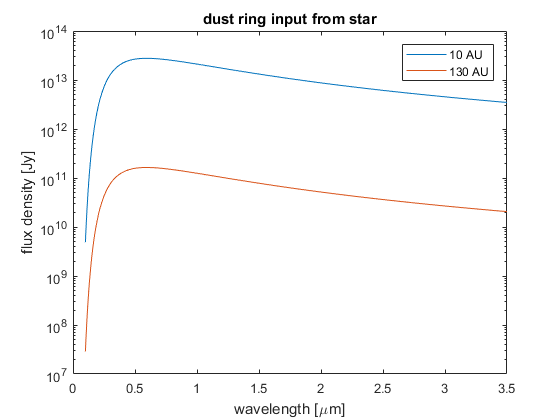
\includegraphics[scale=1]{plot1.png}
\caption{Stellar output at orbital distance}
\end{figure}

\newpage

\section*{Part 2}
The power absorbed by the dust ring in Watts

\begin{tabular}{c|c|c}
& \multicolumn{2}{c}{Orbital radius} \\ 
\hline  
Grain size & 10 AU & 130 AU \\
\hline 
0.1 $\mu$m & $1.463\times 10^{-12}$ & $8.656\times 10^{-15}$ \\ 
\hline 
1 $\mu$m & $6.246\times 10^{-10}$ & $3.696\times 10^{-12}$ \\ 
\hline 
10 $\mu$m & $6.602\times 10^{-8}$ & $3.907\times 10^{-10}$ \\ 
\hline 
1 mm & $7.121\times 10^{-4}$ & $4.214\times 10^{-6}$ \\ 
\hline 

\end{tabular} 

\newpage

\section*{Part 3}
\begin{figure} [h]
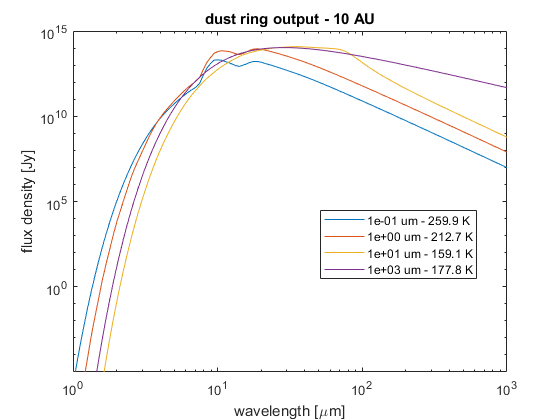
\includegraphics[scale=1]{plot301.png}
\caption{Dust ring output at 10 AU}
\end{figure}

\begin{figure} [h]
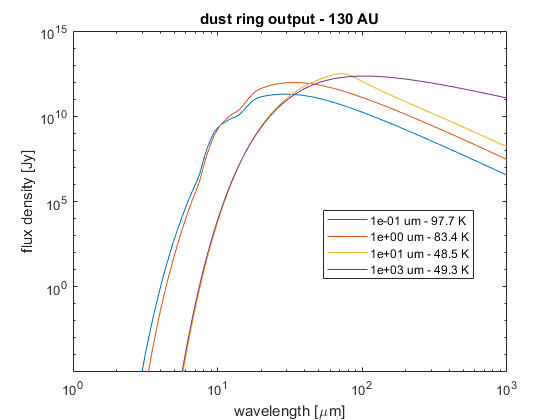
\includegraphics[scale=1]{plot302.png}
\caption{Dust ring output at 130 AU}
\end{figure}


\clearpage
\newpage
\mbox{~}
\clearpage
\newpage

\section*{Part 4}
\begin{figure} [h]
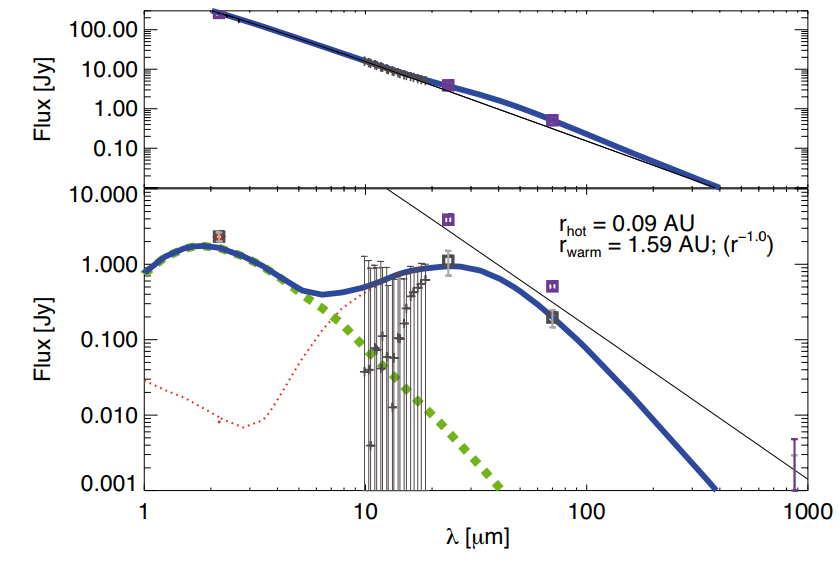
\includegraphics[scale=0.6]{plot4.png}
\caption{SED of Fomalhaut, green: hot ring, red: warm belt, blue: total (Libreton et al., 2013)}
\end{figure}


\newpage

\section*{Part 5}
\begin{tabular}{|c|c|c|c|c|}
\hline 
 & \multicolumn{2}{c|}{10 AU} & \multicolumn{2}{c|}{130 AU} \\ 
\hline 
Grain size & RP & P-R & RP & P-R \\ 
\hline 
0.1 $\mu$m & 4.880 $\times 10^{-21}$ & 2.124$\times 10^{-25}$ & 2.887$\times 10^{-23}$ & 3.486$\times 10^{-28}$ \\ 
\hline 
1 $\mu$ m & 2.083$\times 10^{-18}$ & 9.069$\times 10^{-23}$ & 1.233$\times 10^{-20}$ & 1.488$\times 10^{-25}$ \\ 
\hline 
10 $\mu$ m & 2.202$\times 10^{-16}$ & 9.587$\times 10^{-21}$ & 1.303$\times 10^{-18}$ & 1.573$\times 10^{-23}$ \\ 
\hline 
1 mm & 2.375$\times 10^{-12}$ & 1.034$\times 10^{-16}$ & 1.405$\times 10^{-14}$ & 1.697$\times 10^{-19}$ \\ 
\hline 
\end{tabular} 

\end{document}